\documentclass{article}
\usepackage{amsmath}
\usepackage{xstring}
\usepackage{catchfile}
\usepackage{graphicx}
\usepackage{url}
\usepackage{tikz}
\usepackage{tkz-euclide}
\usepackage[section]{placeins}

\CatchFileDef{\headfull}{../../.git/HEAD}{}
\StrGobbleRight{\headfull}{1}[\head]
\StrBehind[2]{\head}{/}[\branch]
\IfFileExists{../../.git/refs/heads/\branch}{%
    \CatchFileDef{\commit}{../../.git/refs/heads/\branch}{}}{%
    \newcommand{\commit}{\dots~(in \emph{packed-refs})}}
\newcommand{\gitrevision}{%
  \StrLeft{\commit}{7}%
}

\title{Codec 2 Rate K Resampler}
\author{David Rowe\\ \\ Revision: {\gitrevision} on branch: {\branch}}
\date{\today}
\begin{document}

\maketitle

\section{Introduction}

To efficiently transmit spectral amplitude information Codec 2 700C uses a set of algorithms collectively denoted \emph{newamp1}. One of these algorithms is the Rate K resampler which transforms the variable length vectors of spectral amplitude samples to fixed length $K$ vectors suitable for vector quantisation.  This document was written in order to explore and possibly improve rate $K$ resampling.

\section{Theoretical Model}

Consider a vector $\mathbf{a}$ of $L$ spectral amplitudes, sampled at time $t=nT$ seconds, where $n$ is the frame number, and $T$ is the frame period, typically $T=0.01$ seconds. 
\begin{equation}
\mathbf{a} = \begin{bmatrix} A_1, A_2, \ldots A_L \end{bmatrix} 
\end{equation}
$A_m$ is sampled at the frequency $f_m=mF0$ Hz for $m=1 \ldots L$, where $F0$ is the fundamental frequency (pitch) in Hz of the current frame, and $L$ is given by:

\begin{equation}
L=\left \lfloor \frac{F_s}{2F0} \right \rfloor
\end{equation}
$F0$ and $L$ are time varying as the pitch track evolves over time. For speech sampled at $F_s=8$ kHz $F0$ is typically in the range of 50 to 400 Hz, giving $L$ in the range of 10 $\ldots$ 80. \\

To quantise and transmit $\mathbf{a}$, it is convenient to resample $\mathbf{a}$ to a fixed length $K$ element vector $\mathbf{b}$ using a resampling function:
\begin{equation}
\begin{split}
\mathbf{y} &= \begin{bmatrix} Y_1, Y_2, \ldots Y_L \end{bmatrix} = H(\mathbf{a}) \\
\mathbf{b} &= \begin{bmatrix} B_1, B_2, \ldots B_K \end{bmatrix} = R(\mathbf{y})
\end{split}
\end{equation}
Where $H()$ is a filter function chosen to smooth the spectral amplitude samples $A_m$ while not significantly altering the perceptual quality of the speech; and $R()$ is a resampling function. To model the response of the human ear $B_k$  are sampled on $K$ non-linearly spaced points on the frequency axis:
\begin{equation}
\begin{split}
f_k &= warp(k,K) \ \textrm{Hz} \quad k=1 \ldots K \\
warp(1,K) &= 200 \ \textrm{Hz} \\
warp(K,K) &= 3700 \ \textrm{Hz}
\end{split}
\end{equation}
where $warp()$ is a frequency warping function. Codec 2 700C uses $K=20$, and $warp()$ is defined using the Mel function \cite[p 150]{o1997human} (Figure \ref{fig:mel_fhz}) which samples the spectrum more densely at low frequencies, and less densely at high frequencies:
\begin{equation} \label{eq:mel_f}
mel(f) = 2595log_{10}(1+f/700)
\end{equation}
The inverse mapping of $f$ in Hz from $mel(f)$ is given by:
\begin{equation} \label{eq:f_mel}
f = mel^{-1}(x) = 700(10^{x/2595} - 1);
\end{equation}

\begin{figure}[h]
\caption{Mel function}
\label{fig:mel_fhz}
\begin{center}
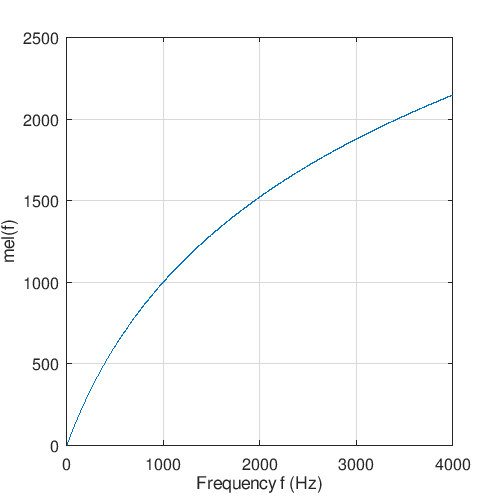
\includegraphics[width=8cm]{ratek_mel_fhz}
\end{center}
\end{figure}

We wish to use $mel(f)$ to construct $warp(k,K)$, such that there are $K$ evenly spaced points on the $mel(f)$ axis (Figure \ref{fig:mel_k}).  Solving for the equation of a straight line we can obtain $mel(f)$ as a function of $k$, and hence $warp(k,K)$ (Figure \ref{fig:warp_fhz_k}):
\begin{equation} \label{eq:mel_k}
\begin{split}
g &= \frac{mel(3700)-mel(200)}{K-1} \\
mel(f) &= g(k-1) + mel(200)
\end{split}
\end{equation}
Substituting (\ref{eq:f_mel}) into the LHS:
\begin{equation} \label{eq:warp}
\begin{split}
2595log_{10}(1+f/700) &= g(k-1) + mel(200) \\
f = warp(k,K) &= mel^{-1} ( g(k-1) + mel(200) ) \\
\end{split}
\end{equation}
and the inverse warp function:
\begin{equation} \label{warp_inv}
k = warp^{-1}(f,K) = \frac{mel(f)-mel(200)}{g} + 1
\end{equation}

\begin{figure}[h]
\caption{Linear mapping of $mel(f)$ to Rate $K$ sample index $k$}
\vspace{5mm}
\label{fig:mel_k}
\centering
\begin{tikzpicture}
\tkzDefPoint(1,1){A}
\tkzDefPoint(5,5){B}
\draw[thick] (1,1) node [right]{(1,mel(200))} -- (5,5) node [right]{(K,mel(3700))};
\draw[thick,->] (0,0) -- (6,0) node [below]{k};
\draw[thick,->] (0,0) -- (0,6) node [left]{mel(f)};
\foreach \n in {A,B}
  \node at (\n)[circle,fill,inner sep=1.5pt]{};
\end{tikzpicture}
\end{figure}

\begin{figure}[h]
\caption{$warp(k,K)$ function for $K=20$}
\label{fig:warp_fhz_k}
\begin{center}
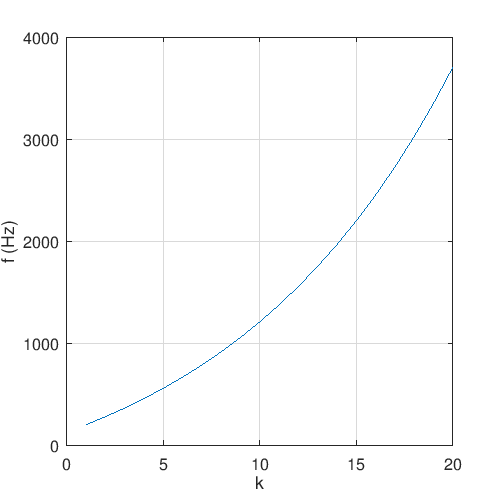
\includegraphics[width=8cm]{warp_fhz_k}
\end{center}
\end{figure}

The rate $K$ vector $\mathbf{b}$ is vector quantised for transmission over the channel:
\begin{equation}
\hat{\mathbf{b}} = Q(\mathbf{b})
\end{equation}
The rate filtered rate $L$ vector can then be recovered by resampling $\mathbf{\hat{b}}$ using another resampling function:
\begin{equation}
\hat{\mathbf{y}} = S(\hat{\mathbf{b}})
\end{equation}
A useful error metric is the mean square error:
\begin{equation} \label{eq:E1}
\begin{split}
E & =\frac{1}{L_{max}-L_{min}+1}\sum_{m=L_{min}}^{L_{max}}(Y_m-\hat{Y}_m)^2 \\
L_{min} & = round(200/F0) \\
L_{max} & =\left \lfloor 3700/F0  \right \rfloor
\end{split}
\end{equation}
In the case where there is no filtering (e.g. \url{newamp1}) then:
\begin{equation}
\begin{split}
H(\mathbf{x}) &= \mathbf{x} \\
\mathbf{y} &= \mathbf{a} \\
\hat{\mathbf{a}} &= \hat{\mathbf{y}} \\
E &=\frac{1}{L_{max}-L_{min}+1}\sum_{m=L_{min}}^{L_{max}}(A_m-\hat{A}_m)^2 
\end{split}
\end{equation}
If $A_m$ are in dB, $E$ can be denoted the spectral distortion in $\textrm{dB}^2$, which can be averaged over a testing database of $N$ frames to obtain mean spectral distortion.

Consider a choice of $warp()$ with linear (non-warped) sampling of the frequency axis, no filtering such that $H(\mathbf{x})=\mathbf{x}$, and an ideal quantiser $Q$ such that $\hat{\mathbf{b}} = \mathbf{b}$. If $K<L$ information may be lost due to undersampling, which implies $\hat{\mathbf{a}} \neq \mathbf{a}$.  
With nonlinear sampling, there will be local undersampling where the sampling rate of $\mathbf{b}$ is less than that of $\mathbf{a}$:
\begin{equation} \label{eq:local_undersampling}
warp(k+1,K)-warp(k,K) < F0
\end{equation}
If $A_m$ is changing rapidly, undersampling may introduce undesirable aliasing, which may manifest as noise that is superimposed on $\mathbf{b}$. This noise may reduce perceptual quality and consume valuable quantiser bits for no benefit. Therefore $H()$ should be chosen to smooth high frequency detail such that local undersampling and uncontrolled aliasing is minimised. This may be restated as choosing $H()$ to minimise $E$ (\ref{eq:E1}) when $\hat{\mathbf{b}} = \mathbf{b}$.

\section{Suggested Experiments}
 
Here are a suggested set of experiments to evaluate the ideas presented in this document.  Some of them require informal listening tests, others have objective measures which could be used as the basis for automated tests:

\begin{enumerate}

\item The baseline resampling (currently a 2nd order polynomial) is a potential source of distortion.  Conduct an experiment to test the theory that $E$ is small (and perceptual quality high) for $K>L$ using linear frequency sampling, $H(\mathbf{x})=\mathbf{x}$ and large $K$.

\item How to demonstrate aliasing?  Well we can run current rate K code, that uses a 2nd order parabolic resampler.  Then compare with a "better" resampler that uses filtering.  Perform an informal listening test over a small set of samples.  Goal is to show reduced $E$ with similar perceptual quality.  Smoothing does reduce information so there will be a trade off.  Too much smoothing and perceptual quality will reduce.  We shoMel-frequency cepstral coefficients (MFCCs)uld also notice improved VQ performance, as we won't be quantising noise.

\item A useful property is sensitivity to quantisation, which could be defined as $\frac{\partial E}{\partial \mathbf{b}}$. For example, given a 1dB RMS error in the elements of $\mathbf{b}$, what is the impact on $E$?

\item To minimise bit rate, it is common to transmit $\mathbf{b}$ to the receiver at period $T/D$ seconds, where $D$ is the decimation ratio, and discarding the intermediate $D-1$ frames. A useful property is the ability to smoothly interpolate between transmitted frames $\mathbf{b}_n$ and $\mathbf{b}_{n+D}$ to recover $\mathbf{b}_{n+i}$ where $i=1 \ldots D-1$.  Need a definition for smoothness.

\item Speech evolves slowly over time compared to the $T=0.01$ second frame period.  Adjacent frames of speech parameters such as $\mathbf{a}_n$ and $\mathbf{a}_{n+1}$ have some correlation which can be used to obtain coding efficiency:
\begin{equation} \label{eq:delta}
\begin{split}
\mathbf{b}_{n+1} & = \mathbf{b}_{n} + \mathbf{\Delta}_n \\
\mathbf{\Delta}_{n+1} & = \mathbf{b}_{n+1} - \mathbf{b}_{n}
\end{split}
\end{equation}

In general $\mathbf{\Delta}_n$ can be encoded with less bits than $\mathbf{b}_n$.  However consider the case where there is significant noise due to undersampling:
\begin{equation}
\mathbf{\hat{b}}_n = \mathbf{b}_{n} + \mathbf{n}_{n}
\end{equation}
where $\mathbf{n}_{n}$ is a vector of noise samples with an unknown distribution. Substituting into (\ref{eq:delta}):
\begin{equation}
\mathbf{\Delta}_{n+1} = \mathbf{b}_{n+1} - \mathbf{b}_{n} + \mathbf{n}_{n+1} - \mathbf{n}_{n}
\end{equation}
If $\mathbf{n}_{n}$ and $\mathbf{n}_{n+1}$ are not well correlated they may become a significant source of noise that is summed with $\mathbf{\Delta}_{n}$, reducing the effectiveness of the quantiser that will need to waste bits quantising the noise. We would therefore expect that in the absence of undersampling noise, delta coding in time should result in increased quantiser efficiency.

\item Small changes in $\mathbf{a}$ input should result in small changes in $\mathbf{b}$ indicating a lack of sensitivity and undersampling noise in $R$.  If $R$ is sensitive, we may notice VQ choices changing from frame to frame for stationary speech.

\item If the sample rate $K$ is sufficiently high (or bandwidth of $\mathbf{a}$ sufficiently constrained), the actual VQ dimension won't matter.  The decorrelation properties of the VQ will ensure it achieves the same distortion over a range of dimensions.  A large enough dimension $K$ could be chosen to simplify $S$, which could be linear resampling. It would be good to decouple $warp()$ from K.
\end{enumerate}

\section{Experiment 1: rate $K>L$ linear}

This experiment tests the ability to resample perfectly ($E=0$) with $K>L$, no filtering ($H(x)=x$) and linear frequency sampling and was implemented with Octave scripts \path{ratek1_fbf.m} and \path{ratek1_batch.m}.

Figure \ref{fig:ratek1_big_dog_50} illustrates why the resampler choice is important.  In the region of F1, the spectral samples $A_{m}$ are changing quickly.  The parabolic resampler fails to track these changes leading to distortion in a perceptually important feature of the spectrum.  When the resampler is viewed as a filter, this can be interpreted as a low pass response in the parabolic resampler, and is most noticable when $K$ is close to $L$.

\begin{figure}[h]
\caption{Frame 50 of big\_dog sample with $K=40$ just larger than $L=37$, 2nd order parabolic resampler.  Note distortion around F1 at 500 Hz }
\label{fig:ratek1_big_dog_50}
\begin{center}
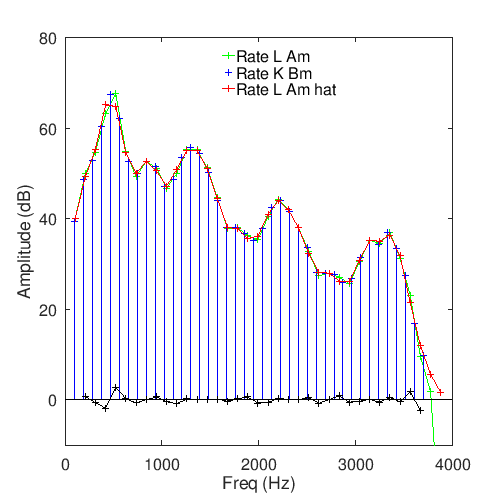
\includegraphics[width=10cm]{ratek1_big_dog_50}
\end{center}
\end{figure}

Figure \ref{fig:ratek1_hts_E} shows the spline and parabolic resampler $E$, plotted against $F0$ for a 24 second sample containing four speakers.  Table \ref{table:ratek1_mean_E} is the mean spectral distortion $E$ over the sample.  The spline interpolator performs better than the parabolic interpolator.  $L$ is time varying, but as it approaches $K$, $E$ increases, once again showing that interpolators struggle with $K$ close to $L$.

\begin{table}[h]
\centering
\begin{tabular}{c c }
 \hline
 Resampler & mean $E$ $\textrm{dB}^2$ \\
 \hline
 spline & 0.02 \\ 
 para  & 0.31 \\
 \hline
\end{tabular}
\caption{Mean spectral distortion $E$ for spline and parabolic interpolators}\label{table:ratek1_mean_E}
\end{table}

In this experiment with $K=80$ both resamplers have low average $E$ (less than $1 \textrm{dB}^2$). On inspection using \url{ratek_fbf} the occasional high $E$ frames were found to be unvoiced speech or background noise, where the pitch estimator tends to return low $F0$ (high $L$) estimates.  Fortunately the ear is quite insensitive to spectral distortion in unvoiced of background noise frames, so it is unlikely these errors are audible.  However with a lower choice of $K$ we would start to get resampling distortion during voiced speech as $K$ approaches $L$ (Figure \ref{fig:ratek1_big_dog_50}), or when $K<L$, aliasing.

\begin{figure}[h]
\caption{Scatter plot of $E$ versus $F0$ for \emph{hts} sample, spline and parabolic resampler}
\label{fig:ratek1_hts_E}
\begin{center}
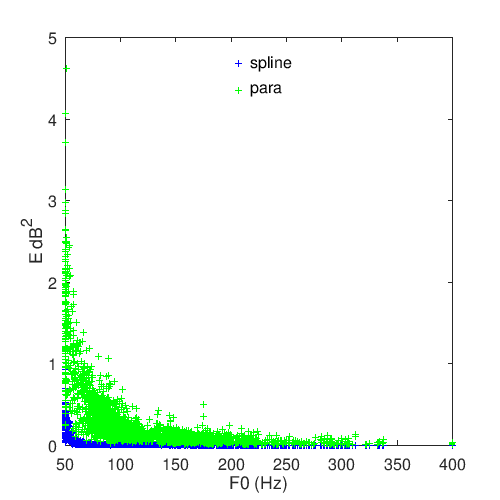
\includegraphics[width=8cm]{ratek1_hts_E.png}
\end{center}
\end{figure}

\begin{figure}[h]
\caption{Histogram of $E$ for spline and parabolic resampler}
\label{fig:ratek1_hts_hist}
\begin{center}
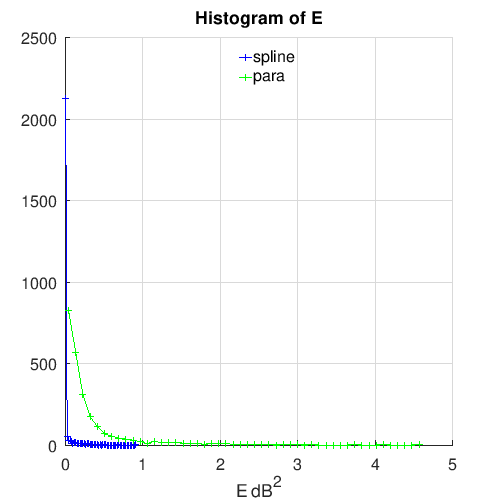
\includegraphics[width=8cm]{ratek1_hts_hist.png}
\end{center}
\end{figure}

Conclusions:
\begin{enumerate}
\item The resampler matters, especially when $K$ is close to $L$.  The current rate $K$ Codec 2 700C system uses $K < L$ (at least at high frequencies) with a parabolic resampler and no filtering.  This may be suffering from resampling noise that affects VQ performance and speech quality. It seems prudent to use a low distortion resampler.  We do not want to add any additional distortion sources to our system.

\item We intend to use $K<L$, which will lead to aliasing distortion.  It would be wise to filter $A_{m}$ prior to resampling to remove the possibility of aliasing and resampler distortion, that is choose $H()$ such that with $\mathbf{b}=\hat{\mathbf{b}}$, $E$ (\ref{eq:E1}) is minimised.

\item Once filtered, there will be some minimum value of $K_{min}$ required for $\mathbf{b}$ such that the rate $L$ vector $\hat{\mathbf{f}}$ can be recovered with minimal $E$. However we are free to choose $K>K_{min}$ as the "bandwidth" of the sampled sequence (and presumably VQ distortion for a given number of bits) will be independent of $K$ when $K>K_{min}$.  While a larger $K$ will use more VQ storage, it may simplify resampling at the receiver.  If $K$ is large enough, a simple linear resampler may suffice.

\item With non-linear frequency sampling, we may need a high local rate near F1 to accurately represent sharp formants, especially for males.  There may be other ways to encode this information, for a example a resampling function or VQ that takes into account $F0$ - "sharpening" F1 for low $F0$ speakers.

\item The newamp1 postfilter is an experimentally derived algorithm that raises peaks and lowers troughs in the rate $K$ spectrum, effectively "sharpening" formants.  When used after vector quantisation it has a large impact on Codec 2 700C speech quality, especially for male speakers.  However it's function is not well understood and in some cases it may be adding distortion.  The sensitivity of F1 to low $K$ resampling provides some hints as to why the postfilter is required.  Resampler distortion in Figure \ref{fig:ratek1_big_dog_50} distorts F1, which is further degraded by vector quantisation.  An increased sample rate and better resampling may reduce the need for the postfilter.

\end{enumerate}

\section{Experiment 2 - Filtering}

The goal of this experiment is to filter the spectral amplitudes $\mathbf{a}$ such that they can be coarsely resampled without resampling or aliasing errors, and with mimimal impact on the perceptual quality.
The $m$th filtered sample can be obtained by:
\begin{equation}
Y_m = \sqrt{\sum_{k=st}^{en}A_k^2 h(k)}
\end{equation}
where $A_k$ is the $k$th \emph{linear} harmonic amplitude, $h(k)$ is sequence of samples defining a suitable filter, and $st$ and $en$ define the start and end harmonics used as input to the filtering operation for the $m$th sample.  This formulation filters the harmonic energies, allowing high amplitude samples (peaks) to contribute more than low amplitude samples. This is an approximation of the ears masking behaviour, and was determined by experiment to slightly improve the peak/trough ratio of formants compared to filtering linear or log (dB) $A_k$.

As we wish to resample on a non-linear frequency axis, we need a set of filters that become wider as frequency increases. We can use the frequency warping function to divide the speech spectrum into $N_b$ bands, with the centre frequency of each band given by:
\begin{equation}
\begin{split}
f_b &= warp(b,N_b) \ \textrm{Hz} \quad b=1 \ldots N_b \\
warp(1,Nb) &= 200 \ \textrm{Hz} \\
warp(Nb,Nb) &= 3700 \ \textrm{Hz}
\end{split}
\end{equation}
For this experiment, we wish to separate the filtering $H()$ from the rate $K$ resampling operation, and perform the filtering on the rate $L$ samples $A_m$.  In this case it is convenient to treat $b$ as a continuous variable.  Given the $m$th harmonic, we can determine the filter band:
\begin{equation}
\begin{split}
f_b &= mF0 \\
b &= warp^{-1}(f_b,N_b) \\
\end{split}
\end{equation}
A triangular function for $g(k)$ has been selected, which tapers to zero in the centre of adjacent bands $b-1$ and $b+1$.  A similar triangular function is used for the filtering stage in the computation of Mel-frequency cepstral coefficients (MFCCs) \cite{davis1980comparison}. This function can be defined in terms of the harmonic indexes, as illustrated in  Figure \ref{fig:triangle_filter}.
\begin{equation}
\begin{split}
st &= max(1,round(warp(b-1,N_b)/F0)) \\
en &= min(L,round(warp(b+1,N_b)/F0)) \\
g(k) &= \frac{k-st}{m-st} \quad k=st \ldots m-1 \\
g(m) &= 1 \\
g(k) &= \frac{en-k}{en-m} \quad k=m+1 \ldots en \\
g_{sum} &= \sum_{k=st}^{en}g(k) \\
h(k) &= g(k)/g_{sum}
\end{split}
\end{equation}
Note the normalising term $g_{sum}$ to ensure the energy of $A_m$ is not altered by the filtering operation. Figure \ref{fig:filters_h} is an example set of filters. It can be seen that $N_b$ controls the filtering.  As $Nb$ becomes smaller, $g(k)$ becomes wider, reducing the rate of change of the filtered spectral samples $Y_m$.  While this presumably improves VQ performance, at some point it will also affect the perceptual quality of the speech.

\begin{figure}[h]
\caption{Triangular Filter $h(k)$.  Note asymmetry on linear frequency axis}
\vspace{5mm}
\label{fig:triangle_filter}
\centering
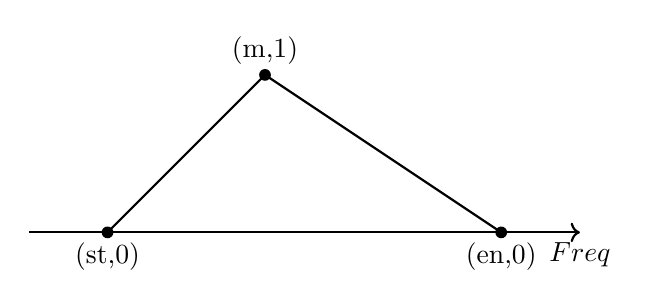
\begin{tikzpicture}
\tkzDefPoint(0,0){A}
\tkzDefPoint(2,2){B}
\tkzDefPoint(5,0){C}
\draw[thick] (0,0) node [below]{(st,0)} -- (2,2) node [above]{(m,1)};
\draw[thick] (2,2) -- (5,0) node [below]{(en,0)};
\draw[thick,->] (-1,0) -- (6,0) node [below]{$Freq$};
\foreach \n in {A,B,C}
  \node at (\n)[circle,fill,inner sep=1.5pt]{};
\end{tikzpicture}
\end{figure}

\begin{figure}[h]
\caption{Filters $h(k)$ for $N_b=10, m=1 \ldots L, F0=200 \textrm{Hz}, L=20$.  There is no smoothing (length 1 filters) up to 1000 Hz, higher frequencies have progressively more smoothing.}
\label{fig:filters_h}
\begin{center}
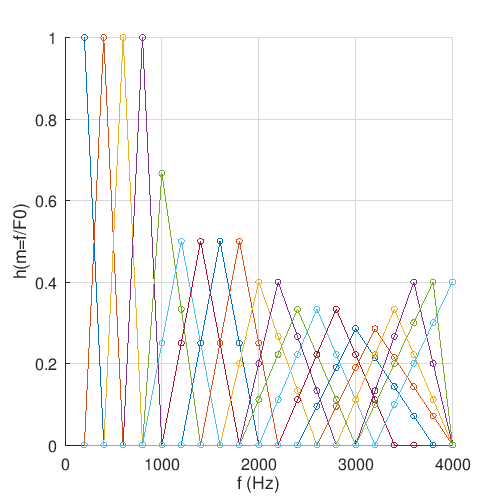
\includegraphics[width=8cm]{filters_h.png}
\end{center}
\end{figure}

Figure \ref{fig:ratek2_E_K_hts} illustrates the effect of varying $K$ for a family of filters by attempting to recover $\hat{\mathbf{y}} = S(R(\mathbf{y}))$ where $\mathbf{y}=H(\mathbf{a})$. As suggested in the conclusion of Experiment 1, once $K>K_{min}$, $\hat{\mathbf{y}}$ can be recovered with very low distortion $E$, even though $K<L$ for many frames.

As $N_b$ increases, the filter width reduces such that $h(k)=1$ for $k=m$ and $h(k)=0$ for $k\ne m$. Thus $N_b=100$ (where $N_b=100 > L_{max}$=80) corresponds to no filtering.  As expected, with $N_b=100$ there is a large spectral distortion $E$ due to undersampling.

Informal listening tests were conducted (3 samples, headphones, spline interpolator, \url{c2sim} tool) with $A_m={\hat{Y}_m}$ to determine the subjective effects of filtering. For $N_b \geq 20$, the speech quality is not significantly affected.  For $N_b \leq 15$ the speech became muffled and harder to understand, presumably as the formants become less well defined.  The filters have the unfortunate property of reducing the spectral peak/trough ratio which the human ear uses to perceive speech (Figure \ref{fig:ratek2_nb_big_dog_50}).  A better smoothing function would preserve the peak/trough ratio of formants, while reducing only the frequency resolution (location and width of formants on the frequency axis). 

\begin{figure}[h]
\caption{Frame 50 of \emph{big\_dog}, plot of filter output $\mathbf{y}$ for $Nb=10$ and $Nb=20$.  Peak to trough ratio decreases with $Nb$, reducing intelligability}
\label{fig:ratek2_nb_big_dog_50}
\begin{center}
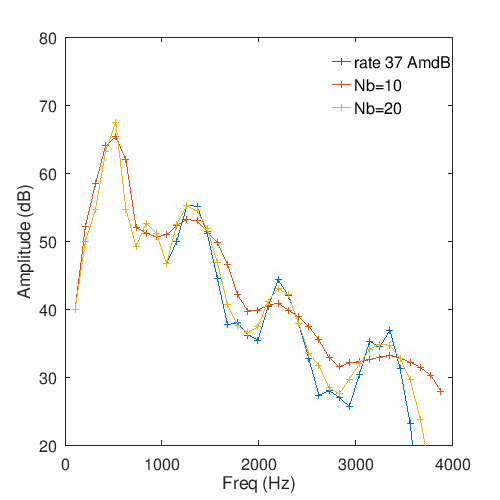
\includegraphics[width=8cm]{ratek2_nb_big_dog_50.png}
\end{center}
\end{figure}

It was also noted that even for $N_b=100$, the speech quality was not significantly affected, despite the high objective distortion evident in Figure \ref{fig:ratek2_E_K_hts} for $Nb=100$.  This is puzzling, as there is significant difference between $\hat{\mathbf{y}}$ and $\mathbf{y}$ due to the aliasing from the rate K resampling $R()$, especially at high frequencies where condition (\ref{eq:local_undersampling}) is not met.  This suggests that the ear is insensitive to noise in the high frequency region, which could be exploited during quantisation to optimise bit allocation.

\begin{figure}[h]
\caption{Mean spectral distortion $E$ against $K$ for a family of filters $H()$ for the 24 second \emph{hts} sample. $N_b=100$ corresponds to no filtering $H(x)=x$, the \emph{para} case is equivalent to the \emph{newamp1} algorithm rate K resampler.}
\label{fig:ratek2_E_K_hts}
\begin{center}
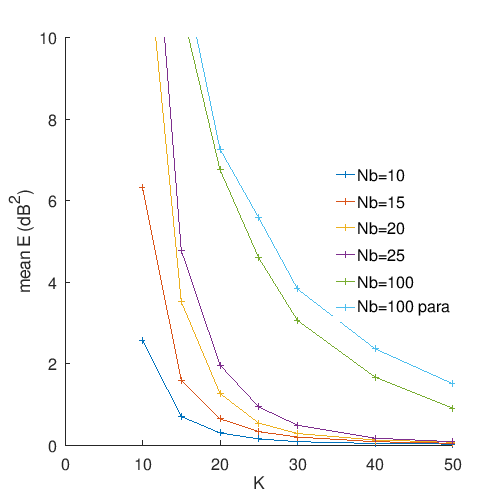
\includegraphics[width=10cm]{ratek2_E_K_hts.png}
\end{center}
\end{figure}

Consider the rate $K$ vectors obtained with ($\mathbf{b_1}$) and without ($\mathbf{b_2}$) filtering:
\begin{equation}
\begin{split}
\mathbf{b_1} &= R(H(\mathbf{a})) \\
\mathbf{b_2} &= R(\mathbf{a}) \\
\mathbf{b_2} &= R(H(\mathbf{a})) + N(\mathbf{a})
\end{split}
\end{equation}
where $N(\mathbf{a})$ is the noise created by local undersampling of $\mathbf{a}$.  If $N(\mathbf{a})$ is even partially uncorrelated with $R(H(\mathbf{a}))$, we would expect to use more bits to quantise $\mathbf{b_2}$ than $\mathbf{b_1}$ to a given level of quantiser distortion $E_q$ given by:
\begin{equation}
E_q =\frac{1}{K}\sum_{k=1}^{K}(b_k-\hat{b}_k)^2 
\end{equation}

An experiment was conducted to train a two stage VQ (mean removed) with and without filtering, the results are presented in Table \ref{table:ratek2_vq} and Figure \ref{fig:20_100_vq}.  A 120 second sample (12000 frames) was used to train the VQ. This VQ design and training material is similar to that used for Codec 2 700C.  These results suggest that the lack of aliasing noise ($N_b=20$) results in a smaller quantiser distortion $E_q$ for a given bit allocation.

\begin{table}[h]
\centering
\begin{tabular}{c c c}
 \hline
 Filter & mean $E_q$ $\textrm{dB}^2$ & RMS $E_q$ dB \\
 \hline
 $N_b=20$ & 3.44 & 1.85 \\ 
 $N_b=100$ (no filtering) & 5.77 & 2.40 \\
 \hline
\end{tabular}
\caption{Spectral distortion for 18 bit, 2 stage, mean removed VQ, with $K=30$}
\label{table:ratek2_vq}
\end{table}

Figure \ref{fig:train_120_Nb20_K30_vq} compares the Kmeans and LBG algorithms for VQ training.  Kmeans initialises the $M=512$ size VQ with random samples from the training set, then performs Kmeans iterations until a distortion metric is met. LBG trains a $M=1$ (0 bit) VQ, then splits and Kmeans trains to get $M=2$ (1 bit), and repeats the process until the final $M=512$ size VQ is obtained.  For this training set, both algorithms arrive at approximately the same final spectral distortion.

In Figure \ref{fig:20_100_vq} and Figure \ref{fig:train_120_Nb20_K30_vq} we note the 2nd stage performs quite poorly, there appears to be step change in the stage 2 gradient compared to the stage 1.  The \emph{mbest} multi-stage search algorithm was tried  (using $mbest=5$ survivors from the first stage) but provided no improvements in $E_q$. These results suggest:

\begin{enumerate}

\item The residual error from stage 1 may be a set of K independent Gaussians, with very little correlation between them.  Intuitively, it makes sense that the first VQ stage would train to make the stage 1 residual error variance in each vector element similar.  Exploring the residual vectors in \url{Octave} shows this is indeed the case - zero mean Gaussian shaped histograms with variances around 7 dB$^2$ for most elements (curiously $k=1$ and $k=30$ higher at 9 and 12 dB$^2$).

\item The $E_q$ after second stage VQ will reduce slowly as the number of bits increases.  

\item The size of $K$ will then be important - it takes more bits to quantise a vector of $K+1$ independant Gaussians than a vector of size $K$.  This is unlike the first stage (and the theory elsewhere in this study) which states $K>K_{min}$ will have little impact on VQ performance as the information (frequency content) in the vector is the same.
 
\item A larger single stage VQ may be a better choice.  Interpolating the Figure \ref{fig:20_100_vq} first stage line, a 12 bit single stage VQ would achieve a similar $E_q$ to the 18 bit two stage VQ.  It would still be feasible to store and search this VQ on a small machine (the entries in dB could be quantised to 8 bits/element, $K2^{12}=123$ kbytes).

\item A two stage VQ with smaller $K$, with a trade off between resampler and VQ distortion.  With smaller $K$, we would expect the second stage $Eq$ to reduce for a given number of bits.

\item Other possibilities are a bug in this analysis (or the software tools), perhaps due to the small size of the training database. 

\item An alternative quantiser based on PCA or DCT rather than direct VQ of $\mathbf{b}$.  Consider a DCT of $\mathbf{b}$ followed by a DCT. The residual into a second stage would still likely be K Gaussians of similar variance, so may suffer the same poor second stage performance.  A method that reduces the dimension of the Gaussians being quantised by the second stage VQ would be useful.

\end{enumerate}

\begin{figure}[h]
\caption{Mean VQ spectral distortion $E_q$ against VQ size in bits for $Nb=20$ and $Nb=100$.  Note the slope of the second stage indicates it performs quite poorly.}
\label{fig:20_100_vq}
\begin{center}
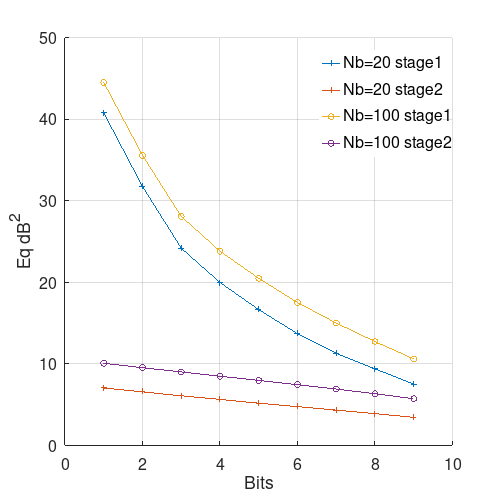
\includegraphics[width=8cm]{20_100_vq.png}
\end{center}
\end{figure}

\begin{figure}[h]
\caption{Kmeans and LBG VQ training for $Nb=20$, very similar results for this training set.}
\label{fig:train_120_Nb20_K30_vq}
\begin{center}
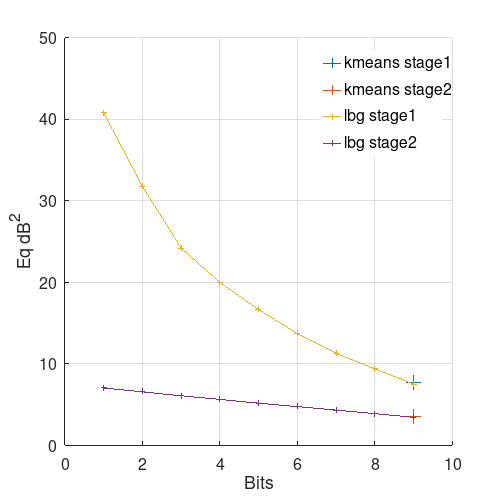
\includegraphics[width=8cm]{train_120_Nb20_K30_vq.png}
\end{center}
\end{figure}

\section{Efficient Filtering}

As $L$ is time varying, it is necessary to determine the filters $g(k)$ for every frame which is computationally inefficient.  A more efficient procedure is to resample $\mathbf{a}$ to rate $L_{high}=L_{max}$ vector $\mathbf{x}$ using the resampler $T()$, perform the filtering $G()$ at rate $L_{high}$, then resample $R()$ to the non-linearly spaced rate $K$ vector $\mathbf{b}$.  This allows $g(k)$ to be precomputed for rate $L_{high}$.  The process now becomes:

\begin{equation}
\begin{split}
\mathbf{x} &=T(\mathbf{a}) \\
\mathbf{y} &= H(\mathbf{x}) \\
\mathbf{b} &= R(\mathbf{y}) \\
\hat{\mathbf{b}} &= Q(\mathbf{b}) \\
\hat{\mathbf{y}}^L &= S(\hat{\mathbf{b}})
\end{split}
\end{equation}

where $\hat{\mathbf{y}}^L$ is sampled at rate $L$, unlike $\mathbf{y}$ which is sampled at rate $L_{high}$.  Note that for the purpose of calculating spectral distortion $E$ it may be covenient to configure $S()$ to extract $\hat{\mathbf{y}}^{Lhigh}$ at rate $L_{high}$.

In Figure \ref{fig:ratek2_E_K_hts}, the \emph{Nb=20 eff} curve shows the results of the efficient filtering algorithm with $\hat{\mathbf{b}} = \mathbf{b}$, which as expected, are very close to the \emph{Nb=20} curve.

\section{Vector Quantiser Training}

Using the algorithms developed above, the 24 minute (144,000 frame) \emph{train.spc} sample was used to train several vector quantisers (Table \ref{table:train_vqs}).  Each frame was resampled to rate $L_{high}$, $N_b=20$ filtered, and resampled to a training set of rate $K=30$ vectors. The spectral distortion $E_q$ results for the single stage VQ were disappointing, however the two stage VQ appears to perform quite well, and is a candidate for an improved 1200 bit/s Codec 2 mode.  As a sanity check, two 4 second samples from within the training set (\emph{big\_dog} and \emph{two\_lines}) were tested with results consistent with the entire training data set.

\begin{table}[h]
\centering
\begin{tabular}{c c c c}
 \hline
 Sample & Vector Quantiser & $E_q$ $\textrm{dB}^2$ & RMS $E_q$ dB \\
 \hline
 train.spc & 1 x 12 bit & 4.84 & 2.20 \\ 
 train.spc & 2 x 12 bit & 1.7 & 1.3 \\
 big\_dog & 2 x 12 bit & 2.03 & 1.43 \\
 two\_lines & 2 x 12 bit & 2.04 & 1.43 \\
 \hline
\end{tabular}
\caption{Spectral distortion for vector quantisers trained using \emph{train.spc}}
\label{table:train_vqs}
\end{table}

\begin{figure}[h]
\caption{Two stage VQ of frame 61 of \emph{big\_dog} (male) }
\label{fig:vq_2stage_big_dog_61}
\begin{center}
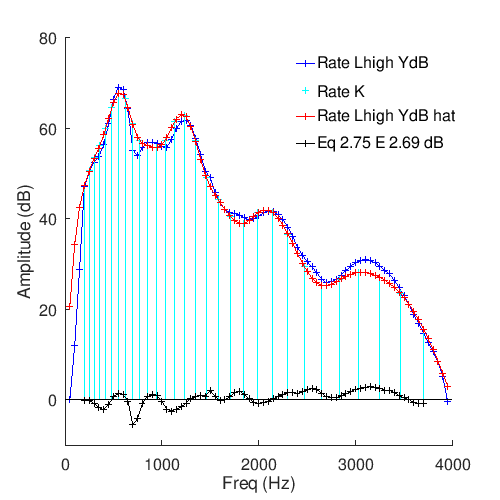
\includegraphics[width=8cm]{vq_2stage_big_dog_61.png}
\end{center}
\end{figure}

\begin{figure}[h]
\caption{Two stage VQ of frame 61 of \emph{two\_lines} (female) }
\label{fig:vq_2stage_two_lines_61}
\begin{center}
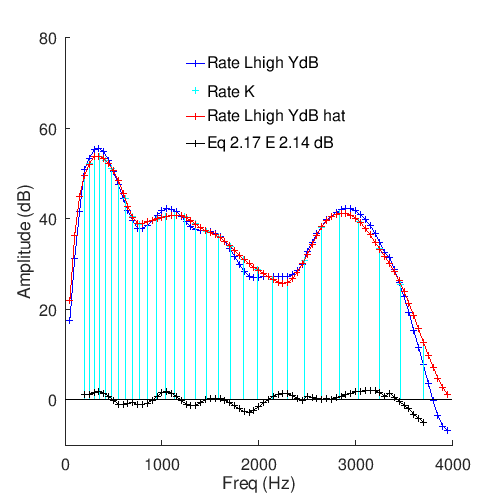
\includegraphics[width=8cm]{vq_2stage_two_lines_61.png}
\end{center}
\end{figure}

\FloatBarrier

\section{Pitch Dependant Spectral Envelope}

Figures \ref{fig:ratek7_big_dog_61} and \ref{fig:ratek7_two_lines_61} overlay the speech spectrum and the corresponding upsampled and filtered rate $L_{high}$ vector $\mathbf{y}$.

When $L<K$ (e.g. females), there are many interpolation functions that result in a low $E$ fit.  It has been observed that for some frames the peaks in $\mathbf{y}$ do not correspond to the peaks in the speech spectrum.  This is acceptable if the quantisation error is small ($\hat{\mathbf{b}}\approx\mathbf{b}$) as the sequence $\mathbf{y}$ can be reconstructed at any interpolated point.  However it suggests that $\mathbf{y}$ may be pitch dependant, requiring separate VQ entries to represent essentially the same spectral information from different $F0$ frames, thus increasing the overall bit rate for a given speech quality.

With low $F0$ males, we note $\mathbf{y}$ is also carrying information about the bandwidth of the peak that is not present for high $F0$ speakers. Narrow bandwidth peaks (in particular F1), have been shown experimentally to be important for the perception of male speech.  As the bandwidth of F1 broadens, the speech becomes muffled.

Thus with low $F0$ speakers, this also suggests a pitch dependency in the spectral envelope $\mathbf{y}$, and corresponding inefficiency in quantisation.

This pitch dependency explains several results in Codec 2 and the wider literature:
\begin{enumerate}
\item Neural speech synthesis use a feature set equivalent to a small $N_b$, small $K$ $\mathbf{b}$ vectors, and produce very high quality speech.  When attempts were made to synthesise speech directly from this feature set using a sinusoidal model, the result was muffled speech. However a Neural model has the ability to use $F0$ as an input feature:
\begin{equation}
\hat{\mathbf{y}} = F(F0, \mathbf{b}) 
\end{equation}
and thus forms narrow bandwidth formants in the model output $\hat{\mathbf{y}}$ during low $F0$ speech. The function $F()$ is typically non-linear, so the peak/formant ratio of $\mathbf{y}$ can be enhanced on reconstruction in a way not possible with a linear resampler, overcoming the smoothing effect of low $N_b$ filtering. 

\item The Codec 2 \emph{newamp1} algorithm used in Codec 2 700 uses an experimentally derived postfilter that has a large impact in the quality of male speech.  It works by expanding the dynamic range of the rate $K$ spectra (multiplying the rate $K$ samples by a constant, then re-normalising to keep energy constant).  The peak harmonics become higher than adjacent harmonics, effectively narrowing the bandwidth of peaks.

\item The group delay of a harmonic in the centre of narrow bandwidth filter will be larger compared to adjacent harmonics outside of the peak.  If F1 is narrow it will "ring" for longer, and the time domain waveform will not decay completely between pitch periods.  This increases the Peak to Average Power Ratio (PAPR) of the synthesised speech, makes it sound less buzzy, and closer to the input speech waveform.

\end{enumerate}

\begin{figure}[h]
\caption{$\mathbf{y}$ for frame 61 of \emph{big\_dog} (high $L$ male), note narrow peak at F1 }
\label{fig:ratek7_big_dog_61}
\begin{center}
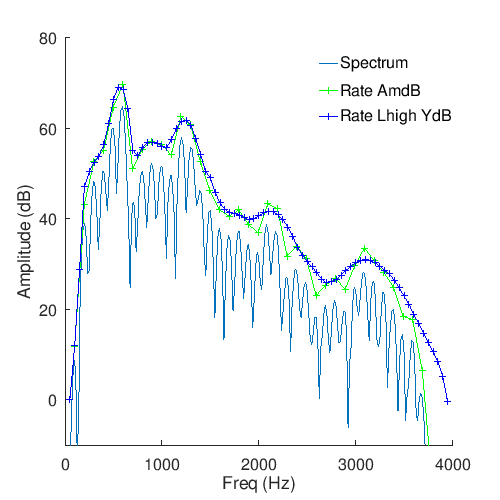
\includegraphics[width=8cm]{ratek7_big_dog_61.png}
\end{center}
\end{figure}

\begin{figure}[h]
\caption{$\mathbf{y}$ for frame 61 of \emph{two\_lines} (low $L$ female), note low frequency peak of $\mathbf{y}$ is not at the same frequency as the spectrum. }
\label{fig:ratek7_two_lines_61}
\begin{center}
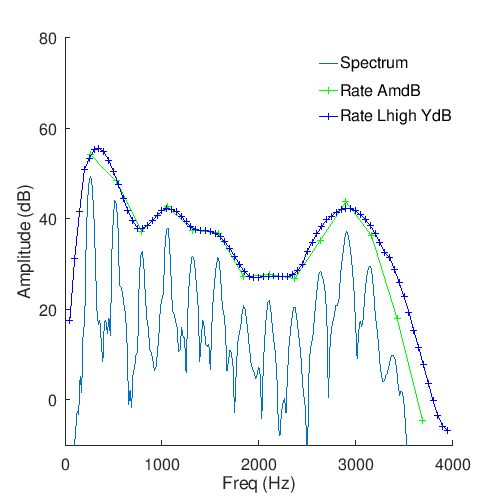
\includegraphics[width=8cm]{ratek7_two_lines_61.png}
\end{center}
\end{figure}

\section{First Pass VQ Listening tests}

Initial listening tests were conducted using a single male (\emph{big\_dog}) and female (\emph{two\_lines}) samples from inside the training dataset and evaluated using headphones.  Samples synthesised with original amplitudes and codec 2 3200 were used as controls.  The \emph{phase0} algorithm was used for all samples to synthesise phases. The female sample sounded quite good under quantisation, however the male sounded buzzy and muffled.

Key observations:
\begin{enumerate}
\item A low frequency artifact, possibly due to reconstruction errors beneath $warp(1,K)$ Hz.  These appeared to go away when a high pass filter was applied to the synthesised speech.
\item Muffled/buzzy, even without vector quantisation, e.g. just filtered and resampled $\hat{\mathbf{y}}^L = S(\mathbf{b})$.  Suggests filtering alone is causing problems, but only for males.
\item Codec 2 3200 sounds fine, this uses a LPC/LSP representation that can accurately model sharp harmonics at all frequencies due to the high bit rate.
\item Application of the \emph{phase0} model with the filtered amplitudes ($\hat{\mathbf{y}}^L = S(\mathbf{b})$) is worse than original phases and the filtered amplitudes.  Use of original phases removes some of the muffled/buzzy effect.  This effect has been observed before.
\item The female sounds fine.
\end{enumerate}

Theory: For low $F0$ speakers, the bandwidth of formants matters at high frequencies, despite the ear having reduced frequency resolution.  We need narrow bandwidth peaks at high frequencies.

Discussion:
\begin{enumerate}
\item The filtering $H()$ broadens high frequency spectral peaks, causing poor quality speech for males. An example can be seen in Figure \ref{fig:ratek7_big_dog_61}, near 2000 and 3000 Hz.
\item A physiological reason based on loudness perception is given in \cite[p 62]{moore97}. For tone pulses of variable duration (2-20ms) but \emph{equal energy}, the probability of detection by a listener is proportional to the tone duration. This suggests \cite{pobloth1999phase} the distribution in time of the energy across a pitch cycle is important. 
\item This effect can be interpreted in terms of the Peak to Average Power Ratio (PAPR) of the speech waveform. For a fixed total energy, the ear prefers speech waveforms with a low PAPR. This has parallels with amplitude compression algorithms such as those for sound recording and analog radio modulation, which also seek to lower the PAPR in order to improve perceptual loudness and intelligibility in high background noise use cases. Several authors \cite{mccree1992improving} \cite{sambur1978reducing} have explored the problem of buzzy and muffled synthesised speech for low $F0$ speakers and noted peakiness (higher PAPR) in the time domain envelope. In the limiting case where all of the pitch cycle energy is concentrated in an impulse (zero phase speech) \cite{xu2017distorting} reported robotic sound quality and decreased intelligibility scores.
\item The theory explains the good results for Codec 2 3200 on the same male.  Due to the high bit rate of this mode we can accurately represent narrow bandwidth peaks at any frequency.  It also explains why the speech quality declines with the lower rate Codec 2 modes that employ LPC/LSPs. They lack the bits to represent the bandwidth of all spectral peaks.
\item As discussed above, representing narrow peaks for low $F0$ male speakers at many frequencies has the potential for VQ inefficiency and an increased bit rate.  A method needs to be found that can preserve the bandwidth of peaks, and still employ a non-linear frequency axis for efficient encoding of the formant centre frequencies.
\item Intuitively, we should be able to represent the speech spectrum with the same number of bits for females as for males.
\item The high quality of speech synthesised from neural networks with low frequency resolution cepstral vectors suggests it is possible to infer or regenerate narrow bandwidth peaks from simpler, lower bit rate (lower $N_b$) spectral representations.  This could be performed via a post filtering algorithm or by training a neural net. 
\item If we use the current low $N_b$ filtering, the post filter should be frequency dependant, only narrowing the bandwidth of high frequency peaks.
\end{enumerate}

Table \ref{table:ratek_phase} summarises the speech quality for a combination of rate $K$ amplitude modelling (\emph{newamp} algorithm) and phase synthesised using the \emph{phase0} model.

\begin{table}[h]
\centering
\begin{tabular}{c c c c}
 \hline
  & Original Phase & Synthesised Phase \\
 \hline
 Original Amplitudes & Good & Good \\ 
 Rate K amplitudes & Good & Poor \\
 \hline
\end{tabular}
\caption{Subjective speech quality for a low pitch male sample with Rate $K$ amplitudes and synthesised phase}
\label{table:ratek_phase}
\end{table}

The \emph{phase0} algorithm fits a minimum phase model to the spectral amplitudes in order to synthesise phase spectra at the decoder.  Near spectral peaks this can be approximated by a second order all pole system with time domain impulse response:
\begin{equation}
x(n)=Ae^{-\alpha n}cos(\omega n)
\end{equation}
$\alpha$ is the time constant that controls the time domain decay of the envelope.  For a wide bandwidth peak $\alpha$ will be large, $x(n)$ will decay quickly and the formant energy will be contained in a shorter period of time.  For a narrow bandwidth peak $\alpha$ will be small and $x(n)$ will decay slowly, the format will "ring" longer and the PAPR will be smaller.

In the frequency domain a small $\alpha$ system results in a rapid phase shift near the peak frequency. If the system is excited by an impulse train (harmonic frequency spectra), a small $\alpha$ results in adjacent harmonics having different phases, and not being aligned in time, shifting time domain energy away from a central peak at the pitch pulse onset.

Group delay is a measure of how long it takes for a tone burst to propagate through a system.  In a minimum phase system, group delay is related to the slope of the frequency response \cite{kates2005principles}.  For a small $\alpha$ (sharper peaks) group delay will be longer, delaying the attack and decay time of the response (mainly energy at the formant centre frequency) to the impulse exciting the system.

This model and the theory above can be used to explain the results in Table \ref{table:ratek_phase}.  With original amplitude we have narrow peaks so the \emph{phase0} algorithm produces a small-$\alpha$ $x(n)$ that rings for some time and sounds natural.  With rate $K$ amplitudes and original phase, we have a phase spectra from the original speech which despite a broad amplitude peak, results in a time domain signal with energy shifted in time from the pitch pulse onset.

With rate $K$ amplitudes and the \emph{phase0} algorithm we have a wide bandwidth amplitude spectra peak that has a small slope near the peak.  Recalling that for minimum phase systems (such as that employed by the \emph{phase0} algorithm), phase shift and group delay are proportional to the slope of the amplitude spectra. Hence adjacent harmonics have small phase shifts, concentrating the energy in time.  Viewed in the time domain, a wide bandwidth means a large-$\alpha$ $x(n)$ again with energy concentrated near the start of the impulse.

The theory also explains why high $F0$ speakers sound better.  Even for broad spectral peaks, the pitch periods are so short that they run together before having a chance to decay.  The ear experiences continuous tones bursts aiding perception of the formant energy.

Possible ways forward:
\begin{enumerate}
\item Raise Nb until males sound OK, design VQ and see how well it works.  May be inefficient, or there may be some correlations across males that VQ can find.
\item Perform filtering on pre-emphasised speech.  Spectral valley energy at frequencies just lower than a high frequency peak can sometimes be higher than the spectral peak due to the slope of the speech spectra.  This can causes reduced spectral peak/valley ratios after filtering.  For an example see the spectral peak of Figure \ref{fig:ratek7_big_dog_61} around 2000 Hz.
\item A freq-dep postfilter.  Need to prove we can narrow formants for males, and enhance peak/valley ratio.
\item A NN is one solution - sharp peaks for males (based on F0), and enhance peaks/valley ratio at high frequencies.  What would we use as ground truth?  Is there a toy example we can train against?  How can we make it handle wide dynamic ranges?  How do we know we have enough training data? Need to see it enhancing indep of frequency of formant - that would be a good test.  Just train on voiced, high energy frames.
\end{enumerate}

\section{Post Filter Design}

We require a function $P()$ that modifies a smoothed vector of spectral magnitude samples $\mathbf{y}$ to sharpen formant peaks and increase peak/valley ratio at high frequencies.

The filter $P()$ is needed for low $F0$ speakers and voiced speech.

The smoothed vector $\mathbf{y}$ is obtained by filtering $\mathbf{y}=H(\mathbf{x})$, where $H()$ is a filter function defined by the parameter $N_b$ that provides progressively more smoothing as frequency increases.  This smoothing reduces the information in $\mathbf{y}$ making it possible to quantise at low bit rates. At low frequencies $H(X_k)=X_k$ therefore $P()$ should modify the spectra only at high frequencies, leaving low frequencies unchanged. 

Representing the sharp peaks required for male speech is possible by direct quantisation of $\mathbf{x}$ but requires a prohibitively high bit rate for our use case.  High $F0$ speakers can be adequately represented by a low $N_b$ vector  which suggests there should be a way to reproduce male speech of adequate quality from low $N_b$ vectors.  $P()$ should have no effect on high $F0$ speakers, which are already adequately represented by the smoothed spectral samples.

\bibliographystyle{plain}
\bibliography{ratek_references}
\end{document}

